% generated by make_combined.py from stage5_practice_theory/stage5.tex; do not edit
\section{Stage 5 --- Practice, breadth and theory}\label{sec:stage5}

\stagebox{\textbf{In one sentence.} On unaltered test sets masking harms exactly the cases the location law says it
should --- shortcut-conflicting images with an in-ROI artifact --- and on the patient-disjoint thyroid split it lowers
sensitivity at every validation-fixed operating point; the crossover replicates in \sFiveNFrozenPos{} of \sFiveNFrozen{}
frozen encoder--cohort pairs, at three model sizes, in \sFiveNFtPos{} of \sFiveNFt{} fine-tuned networks, in the zero-shot
scores of vision--language models, and on new patients (ISIC 2020, \sFiveExtX); a two-parameter linear-Gaussian model
predicts held-out reversed AUROC with mean error \sFiveTMae, less than half the error of the best heuristic, and explains
why the law holds.}
\subsection{Where this stage starts}
Stages~1--4 established the location law in constructed environments --- a strong artifact--label association in
training and its reversal at test --- showed its mechanism (retention with amplified reliance), and showed that it is not
explained by which images carry the artifact. A clinician will ask two questions that this cannot answer: does it
matter on data as collected, without an imposed association, and at the operating point a clinic would use? A
methodologist will ask two more: is the result a property of one encoder and one training regime, and can it be
predicted rather than only observed? This stage answers all four.

\subsection{Questions}
\begin{enumerate}[label=\textbf{Q5\alph*},leftmargin=*]\itemsep1pt
\item On natural test sets, does masking harm the shortcut-conflicting cases, and does that change clinical
sensitivity at fixed operating points?
\item How broadly does the crossover replicate: encoder families and sizes, end-to-end fine-tuning, untrained
(zero-shot) models, new patients?
\item Can a simple model predict a model's reversed-test AUROC from what is observable without the reversed test --- and
so explain when masking helps?
\end{enumerate}
\paragraph{Design decisions} \emph{Hard pairs.} On a natural test set the artifact--label association is weak, so the
overall AUROC barely moves. Positive--negative pairs are therefore split by whether their artifact status conflicts with
the test set's own association (hard) or follows it (easy); the law predicts harm on hard pairs, where the retained
in-ROI artifact points the wrong way. \emph{Operating points fixed on validation data} (never on test) at five clinically
motivated targets, with thresholds re-estimated in every bootstrap replicate. \emph{A theory judged by held-out error,
not by fit}: the model is fitted to each cell's clean and correlated AUROC and must predict the reversed AUROC it never
saw, against two parameter-free heuristics. Rejected: judging the theory by agreement with simulations drawn from its own
assumptions (circular), and by the correlation of predicted and observed crossovers (a heuristic reaches almost the same
correlation).

\subsection{Methods}
\paragraph{Natural test sets} Models are trained on the natural training distribution (no imposed association).
Thyroid: the official patient-disjoint TNCD split \citep{gong2022acl} (614 test images; in-ROI calipers on 37.6\% of benign
and 24.1\% of malignant training images). Dermoscopy: each source (BCN, HAM, MSK) held out in turn (in-lesion hair on 31\%
of melanomas and 20\% of benign lesions). Capsule: held-out frame-block groups. 5 seeds of a group-safe train/validation
split. $A$ = in-ROI artifact. Arms ERM, masking and group balancing.
\paragraph{Clinical metrics and operating points} AUROC, AUPRC, Brier score, expected calibration error; sensitivity and
specificity at OP1--OP5, overall and among shortcut-conflicting positives (for thyroid: malignant nodules with a caliper
on the nodule).
\paragraph{Replication} Frozen DINOv2 ViT-S/B/L (21/86/304\,M parameters), MedSigLIP-448, ConvNeXt-384 and DermLIP with
linear heads; ResNet-50 and ViT-S/16 fine-tuned end to end (ImageNet initialisation, 224\,px, 8 epochs, AdamW, one-cycle
learning rate $10^{-4}$ or $3\cdot10^{-5}$, head $\times10$, thresholds on clean validation; the five folds of seed 42 are
the bootstrap clusters, 15 clusters for the ovary); zero-shot vision--language scores (cosine to a positive minus a
negative class prompt) of MedSigLIP and DermLIP.
\paragraph{External validation} ISIC 2020 \citep{rotemberg2021isic2020} was run only if a gate registered before any
external label was read held: direct download without an agreement, a research licence, patient identifiers, masks
producible by frozen models, and at least 50 images in every cell. Lesion masks: the existing U-Net (ISIC 2018 Task~1
only). Hair masks: a segmenter trained only on the ISIC 2019 hair masks and frozen before any ISIC 2020 image was scored.
Protocol of the ISIC 2019 traps unchanged; groups = patient identifier.
\paragraph{Theory} A frozen encoder maps an image to a disease block with signal-to-noise ratio $S$, an artifact block with
signal-to-noise ratio $A$, and noise. Training uses $P(A{=}1\mid Y{=}1)=p_1=0.9$ and $P(A{=}1\mid Y{=}0)=p_0=0.1$. An
LDA-optimal linear head (which logistic regression approximates) weights each block by its training signal; the
artifact's effective training signal is
\[\tilde A=\frac{(p_1-p_0)^2A}{1+p_1(1-p_1)A},\qquad
\mathrm{AUROC}_{\text{rev}}=\Phi\!\left(\frac{S-\tilde A}{\sqrt{2(S+\tilde A)}}\right),\]
which rises with $S$ and falls with $\tilde A$; for any test composition $q_y=P(A{=}1\mid Y{=}y)$ the same model gives
the AUROC in closed form (\texttt{docs/THEORY.md}). Its consequences: (1) out-of-ROI masking sets $\tilde A\to0$ and helps
unless it destroys most of the disease signal; (2) in-ROI masking keeps $\tilde A$ and changes $S$ to $S_m$, so it
\emph{harms iff it removes disease-informative context} ($S_m<S$); (3) for the same $S_m$ the crossover is positive for
every $\tilde A>0$; (4) group balancing sets the effective association to zero for the artifact and everything
correlated with it, independently of location; (5) a shortcut carried by correlates that the clean and correlated
environments do not reveal is invisible to the model. \emph{Test}: for every cell (result $\times$ trap or overlap
$\times$ arm) $(S,A)$ is fitted to the observed clean and correlated AUROC and the reversed AUROC is predicted; heuristics
``reversed = clean'' and ``symmetric reversal'' (reversed $=$ clean $-$ (correlated $-$ clean)).

\subsection{Experiments}
\begin{table}[H]\centering\scriptsize
\caption{Experiments of this stage and their registration documents (\texttt{docs/PREREGISTRATION\_<name>.md}). Commit times are set by the committing machine and are not independent proof of order.}\label{s5:tab:exp}
\begin{tabular}{p{3.1cm}p{2.1cm}p{2.4cm}p{3.2cm}p{3.3cm}}\toprule
Experiment & Status & Registration & First commit (local time) & Support criterion \\\midrule
Zero-shot vision--language scores, Z1 & \mixed{} registered (descriptive); crossover test post hoc & TEXT\_\allowbreak{}PROMPT & \texttt{7877e8c}, 2026-09-27 12:21 & correlated $-$ reversed gap reported \\
Natural test sets, N3 (hard pairs) & \ok{} registered & NATURAL & \texttt{74bd243}, 2026-09-27 09:39 & mask $-$ ERM $<0$ on hard pairs \\
Operating points S1--S3 & \ok{} registered & REVIEW2 (R3) & \texttt{29cd0da}, 2026-09-27 18:56 & ``masking lowers sensitivity'' only if S1 and $\ge3$ of OP2--OP5 \\
Thyroid subgroup, $n=$\sFiveNConf{} (S3) & \mixed{} registered test in a post hoc subgroup & REVIEW2 (R3) & \texttt{29cd0da}, 2026-09-27 18:56 & sensitivity loss in the subgroup, CI $<0$ \\
Crossed CIs for the subgroup (R6) & \ok{} registered & REVIEW3 (R6) & \texttt{85da735}, 2026-09-27 23:43 & report the crossed CI \\
Fine-tuned hair model and literature comparison (R4) & \ok{} registered & REVIEW2 (R4) & \texttt{29cd0da}, 2026-09-27 18:56 & crossover CI $>0$; comparison descriptive \\
Encoder scale (S/B/L) & \ok{} registered & SCALE & \texttt{13303b0}, 2026-09-27 14:13 & crossover CI $>0$ at every scale \\
Fine-tuned networks & \ok{} registered & FINETUNE & \texttt{7c8b466}, 2026-09-27 07:06 & crossover CI $>0$ (secondary) \\
DermLIP hair traps & \ok{} registered & ISIC2019\_\allowbreak{}TRAPS & \texttt{76e25d4}, 2026-09-26 13:14 & crossover CI $>0$ \\
Theory as held-out predictor, T1--T4 & \ok{} registered & THEORY\_\allowbreak{}PREDICTION & \texttt{4f78653}, 2026-09-27 13:46 & MAE below both heuristics; crossover signs \\
External validation, X1 (ISIC 2020) & \ok{} registered & FINAL (A4) & \texttt{c45d482}, 2026-09-28 00:35 & gate, then crossover CI $>0$ \\
\bottomrule\end{tabular}
\end{table}


\subsection{Results}
\subsubsection{Natural test sets}
Table~\ref{s5:tab:nat}. On all pairs, masking changes little. On shortcut-conflicting pairs it harms in thyroid
(\sFiveNatthyroidhard), BCN (\sFiveNatisicBCNhard) and MSK (\sFiveNatisicMSKhard), and helps in HAM
(\sFiveNatisicHAMhard); in capsule the interval includes zero (\sFiveNatcapsulehard). Where masking harms the hard pairs,
it helps or is neutral on the easy ones (MSK \sFiveNatisicMSKeasy) --- the signature of a model that still uses an in-ROI
artifact after masking: it gets the aligned cases right for the wrong reason and the conflicting cases wrong. The
registered claim N3 is supported in three of five natural test sets. Group balancing improves on masking for the hard
pairs of thyroid (\sFiveNatBalthyroidhard), BCN (\sFiveNatBalisicBCNhard) and MSK (\sFiveNatBalisicMSKhard), but not on
all pairs and not in capsule (\sFiveNatBalcapsuleall{} on all pairs).
\begin{table}[H]\centering\scriptsize
\caption{Natural test sets: AUROC change from masking on all positive--negative pairs and on the pairs whose artifact status conflicts with (``hard'') or follows (``easy'') the test set's own artifact--label association (DINOv2, crossed CIs).}\label{s5:tab:nat}
\resizebox{\linewidth}{!}{\begin{tabular}{lcccc}\toprule
Test set (no imposed correlation) & $P(A{=}1\mid Y{=}1)$ / $P(A{=}1\mid Y{=}0)$ & mask $-$ ERM, all pairs & shortcut-conflicting pairs & shortcut-aligned pairs \\\midrule
Thyroid (official patient-disjoint split) & 0.331 / 0.434 & $-0.004$ [$-0.048, +0.041$] & $-0.095$ [$-0.165, -0.022$] & $+0.042$ [$-0.011, +0.097$] \\
Dermoscopy, BCN held out & 0.356 / 0.239 & $-0.025$ [$-0.035, -0.016$] & $-0.025$ [$-0.043, -0.008$] & $-0.022$ [$-0.035, -0.008$] \\
Dermoscopy, HAM held out & 0.274 / 0.184 & $+0.031$ [$+0.017, +0.045$] & $+0.050$ [$+0.030, +0.070$] & $+0.004$ [$-0.019, +0.027$] \\
Dermoscopy, MSK held out & 0.109 / 0.074 & $+0.016$ [$-0.007, +0.038$] & $-0.065$ [$-0.111, -0.019$] & $+0.100$ [$+0.056, +0.147$] \\
Capsule (held-out frames) & 0.101 / 0.232 & $+0.077$ [$+0.059, +0.097$] & $+0.021$ [$-0.003, +0.048$] & $+0.071$ [$+0.040, +0.108$] \\
\bottomrule\end{tabular}}
\end{table}


\subsubsection{Clinical consequences: thyroid operating points}
On the official, patient-disjoint thyroid test split the AUROC of ERM and of the masked model is almost the same
(\sFiveThyAucerm{} and \sFiveThyAucmask), but masking lowers sensitivity at every operating point (Table~\ref{s5:tab:opthy},
Figure~\ref{s5:fig:op}): at OP1 by \sFiveSensOPOne{} (from \sFiveThySenserm{} to \sFiveThySensmask) and at OP2--OP5 with
intervals below zero in \sFiveNSensLoss{} of 4. By the decision rule registered before the operating points were computed
(S1 and a loss at $\ge3$ of OP2--OP5), the thesis may say that masking lowers sensitivity on this test set. Specificity
rises: masking moves the operating point, and the loss falls on the malignant nodules whose caliper lies on the nodule.
\paragraph{The subgroup of \sFiveNConf{} malignant nodules} \textbf{Registration status: a pre-registered test inside a
post hoc subgroup --- exploratory confirmation.} The subgroup (malignant nodules with an in-ROI caliper) was defined after
the natural-distribution AUROC results were known; the operating-point test in it was registered before the operating
points were computed. The same \sFiveNConf{} nodules enter every seed. At OP2, sensitivity in this subgroup falls from
\sFiveConfErmOPTwo{} to \sFiveConfMaskOPTwo, a change of \sFiveConfOPTwo. The effect is large and consistent across
operating points; its confirmatory weight is limited by the post hoc subgroup definition.
\begin{table}[H]\centering\scriptsize
\caption{Thyroid, official patient-disjoint test split: effect of masking at five validation-fixed operating points (crossed bootstrap with thresholds re-estimated in every replicate). The subgroup is the malignant nodules with an in-ROI caliper (shortcut-conflicting).}\label{s5:tab:opthy}
\resizebox{\linewidth}{!}{\begin{tabular}{lccccc}\toprule
Operating point (fixed on validation) & Sensitivity ERM $\to$ mask & $\Delta$ sensitivity & $\Delta$ specificity & Sensitivity, conflicting malignant (ERM $\to$ mask) & $\Delta$ in that subgroup \\\midrule
OP1 max.\ balanced accuracy & 0.699 $\to$ 0.424 & $-0.275$ [$-0.435, -0.138$] & $+0.202$ [$+0.115, +0.330$] & 0.703 $\to$ 0.223 & $-0.479$ [$-0.640, -0.313$] \\
OP2 specificity $\ge0.80$ & 0.557 $\to$ 0.355 & $-0.202$ [$-0.300, -0.100$] & $+0.117$ [$+0.059, +0.172$] & 0.549 $\to$ 0.177 & $-0.372$ [$-0.499, -0.236$] \\
OP3 specificity $\ge0.90$ & 0.371 $\to$ 0.219 & $-0.152$ [$-0.253, -0.043$] & $+0.075$ [$+0.029, +0.122$] & 0.336 $\to$ 0.100 & $-0.236$ [$-0.383, -0.089$] \\
OP4 sensitivity $\ge0.80$ & 0.753 $\to$ 0.380 & $-0.373$ [$-0.469, -0.270$] & $+0.278$ [$+0.203, +0.359$] & 0.744 $\to$ 0.197 & $-0.546$ [$-0.671, -0.421$] \\
OP5 sensitivity $\ge0.90$ & 0.869 $\to$ 0.588 & $-0.281$ [$-0.391, -0.178$] & $+0.339$ [$+0.236, +0.425$] & 0.862 $\to$ 0.400 & $-0.462$ [$-0.614, -0.310$] \\
\bottomrule\end{tabular}}
\end{table}

\begin{figure}[H]\centering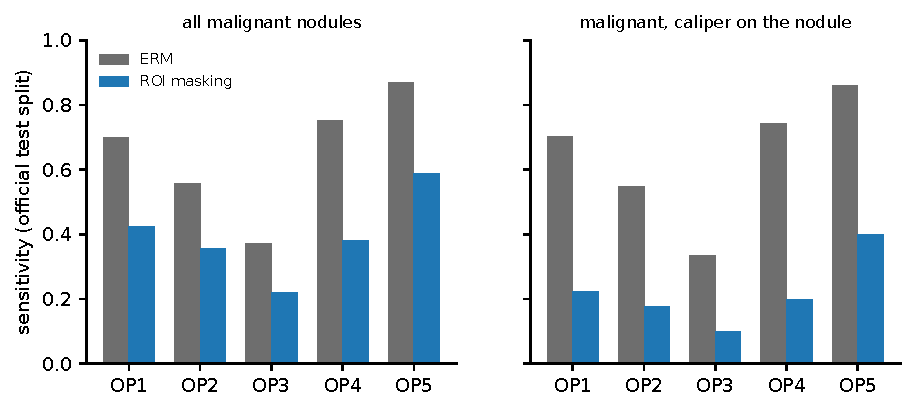
\includegraphics[width=\linewidth]{../stage5_practice_theory/figures/op_thyroid.pdf}
\caption{Thyroid, official patient-disjoint test split: sensitivity of ERM and of the masked model at five
validation-fixed operating points, for all malignant nodules (left) and for the \sFiveNConf{} malignant nodules with a
caliper on the nodule (right; post hoc subgroup, exploratory).}\label{s5:fig:op}\end{figure}
\paragraph{Other test sets} Table~\ref{s5:tab:opother}. At OP2 masking lowers sensitivity, including for the
shortcut-conflicting positives, in the HAM and MSK hold-outs, where it raises specificity; in BCN it lowers specificity; in
capsule it raises sensitivity without a significant change for the conflicting erosions. The thyroid pattern --- a
threshold that no longer catches the positives whose supporting artifact is gone --- recurs in two of the four other
test sets. Table~\ref{s5:tab:clin} gives the threshold-free and
calibration metrics: in thyroid and BCN masking worsens Brier score and calibration; in HAM, MSK and capsule it improves
every metric, matching the AUROC results.
\begin{table}[H]\centering\scriptsize
\caption{Other natural test sets at OP2 (validation specificity $\ge0.80$), mask $-$ ERM, crossed CIs.}\label{s5:tab:opother}
\begin{tabular}{lcccc}\toprule
Test set & Conflicting positives & $\Delta$ sensitivity & $\Delta$ specificity & $\Delta$ sensitivity, conflicting \\\midrule
Dermoscopy BCN & 1832 & $+0.017$ [$-0.003, +0.036$] & $-0.110$ [$-0.135, -0.079$] & $+0.019$ [$-0.004, +0.042$] \\
Dermoscopy HAM & 808 & $-0.062$ [$-0.110, -0.015$] & $+0.092$ [$+0.064, +0.121$] & $-0.055$ [$-0.104, -0.007$] \\
Dermoscopy MSK & 492 & $-0.074$ [$-0.127, -0.026$] & $+0.083$ [$+0.064, +0.110$] & $-0.094$ [$-0.149, -0.044$] \\
Capsule & 38 & $+0.140$ [$+0.082, +0.222$] & $+0.041$ [$-0.029, +0.107$] & $+0.022$ [$-0.041, +0.123$] \\
\bottomrule\end{tabular}
\end{table}

\begin{table}[H]\centering\scriptsize
\caption{Clinical metrics on the natural test sets (seed means; threshold at maximal balanced accuracy on validation data).}\label{s5:tab:clin}
\begin{tabular}{lccccccc}\toprule
Test set & Arm & AUROC & AUPRC & Brier & ECE & Sensitivity & Specificity \\\midrule
Capsule (held-out frames) & ERM & 0.889 & 0.897 & 0.130 & 0.042 & 0.770 & 0.844 \\
 & mask & 0.967 & 0.971 & 0.069 & 0.029 & 0.856 & 0.933 \\
 & balanced & 0.881 & 0.889 & 0.136 & 0.051 & 0.757 & 0.838 \\
ISIC, BCN held out & ERM & 0.786 & 0.587 & 0.238 & 0.279 & 0.842 & 0.521 \\
 & mask & 0.761 & 0.564 & 0.287 & 0.330 & 0.842 & 0.443 \\
 & balanced & 0.782 & 0.587 & 0.229 & 0.260 & 0.835 & 0.509 \\
ISIC, HAM held out & ERM & 0.752 & 0.355 & 0.161 & 0.233 & 0.575 & 0.789 \\
 & mask & 0.782 & 0.396 & 0.138 & 0.199 & 0.569 & 0.831 \\
 & balanced & 0.751 & 0.350 & 0.154 & 0.225 & 0.495 & 0.845 \\
ISIC, MSK held out & ERM & 0.770 & 0.477 & 0.171 & 0.160 & 0.600 & 0.790 \\
 & mask & 0.785 & 0.497 & 0.149 & 0.120 & 0.587 & 0.823 \\
 & balanced & 0.767 & 0.464 & 0.175 & 0.165 & 0.628 & 0.759 \\
Thyroid (official split) & ERM & 0.735 & 0.604 & 0.209 & 0.088 & 0.699 & 0.653 \\
 & mask & 0.731 & 0.629 & 0.215 & 0.119 & 0.424 & 0.856 \\
 & balanced & 0.714 & 0.580 & 0.220 & 0.115 & 0.707 & 0.612 \\
\bottomrule\end{tabular}
\end{table}


\subsubsection{Replication breadth}
Table~\ref{s5:tab:breadth} and Figure~\ref{s5:fig:breadth}. The crossover's interval lies above zero for \sFiveNFrozenPos{} of
\sFiveNFrozen{} frozen encoder--cohort pairs; the exception is DermLIP (Stage~3).
\paragraph{Model scale} Table~\ref{s5:tab:scale}. The law holds at every size in every cohort. Larger models do not escape
the shortcut; they exploit an in-ROI caliper \emph{more}: ERM's correlated$-$reversed gap in the thyroid Trap~A grows
from \sFiveGapthyroidViTS{} (ViT-S) to \sFiveGapthyroidViTB{} (ViT-B) and \sFiveGapthyroidViTL{} (ViT-L), and in the ovary
from \sFiveGapovaryViTS{} to \sFiveGapovaryViTL; capsule is flat.
\begin{table}[H]\centering\scriptsize
\caption{Encoder scale (DINOv2 ViT-S/14 21\,M, ViT-B/14 86\,M, ViT-L/14 304\,M parameters): ERM's shortcut gap in the in-ROI trap and the crossover.}\label{s5:tab:scale}
\begin{tabular}{lcccc}\toprule
Cohort & DINOv2 & ERM clean AUROC (Trap A) & ERM gap corr $-$ rev (Trap A) & Crossover \\\midrule
Thyroid & ViT-S/14 & 0.629 & 0.537 & $+0.247$ [$+0.205, +0.288$] \\
Thyroid & ViT-B/14 & 0.608 & 0.590 & $+0.239$ [$+0.196, +0.280$] \\
Thyroid & ViT-L/14 & 0.601 & 0.622 & $+0.263$ [$+0.218, +0.307$] \\
Ovary & ViT-S/14 & 0.698 & 0.320 & $+0.296$ [$+0.208, +0.384$] \\
Ovary & ViT-B/14 & 0.635 & 0.413 & $+0.170$ [$+0.087, +0.252$] \\
Ovary & ViT-L/14 & 0.608 & 0.564 & $+0.207$ [$+0.127, +0.286$] \\
Capsule & ViT-S/14 & 0.803 & 0.363 & $+0.370$ [$+0.325, +0.415$] \\
Capsule & ViT-B/14 & 0.796 & 0.360 & $+0.377$ [$+0.327, +0.426$] \\
Capsule & ViT-L/14 & 0.820 & 0.347 & $+0.417$ [$+0.369, +0.464$] \\
\bottomrule\end{tabular}
\end{table}

\paragraph{End-to-end fine-tuning} Table~\ref{s5:tab:ftdet}. The crossover replicates in \sFiveNFtPos{} of \sFiveNFt{}
fine-tuned networks: dermoscopy hair with ResNet-50 (\sFiveFtDermoscopyhairResNetFiveZero), thyroid with ViT-S and
capsule with ResNet-50, where masking harms strongly inside the ROI (\sFiveFtACapsuleResNetFiveZero) and helps outside
(\sFiveFtBCapsuleResNetFiveZero). The thyroid ResNet-50 points the same way without significance. The fine-tuned ovary
network is \emph{not evaluable}: with 15 clusters its ERM clean AUROC is \sFiveOvFtCleanA{} (Trap~A) and \sFiveOvFtCleanB{}
(Trap~B) --- it barely learns the task --- so its null says nothing about the law. Fine-tuning does not remove the effect;
it is not an artefact of frozen features.
\begin{table}[H]\centering\scriptsize
\caption{End-to-end fine-tuned networks (ImageNet initialisation, 224\,px, 8 epochs; folds as bootstrap clusters): effect of masking per trap (crossed CIs).}\label{s5:tab:ftdet}
\begin{tabular}{lccc}\toprule
Fine-tuned network & mask $-$ ERM, Trap A & mask $-$ ERM, Trap B & mask+balanced $-$ balanced, Trap A \\\midrule
Dermoscopy hair, ResNet-50 & $-0.002$ [$-0.054, +0.049$] & $+0.141$ [$+0.071, +0.214$] & $-0.008$ [$-0.072, +0.059$] \\
Thyroid, ResNet-50 & $+0.078$ [$+0.032, +0.123$] & $+0.142$ [$+0.073, +0.211$] & $+0.085$ [$+0.035, +0.137$] \\
Thyroid, ViT-S/16 & $+0.122$ [$+0.068, +0.170$] & $+0.244$ [$+0.163, +0.329$] & $+0.059$ [$+0.003, +0.122$] \\
Capsule, ResNet-50 & $-0.279$ [$-0.377, -0.185$] & $+0.327$ [$+0.235, +0.416$] & $-0.020$ [$-0.107, +0.074$] \\
Ovary, ResNet-50 (15 clusters) & $+0.152$ [$+0.070, +0.232$] & $+0.211$ [$+0.090, +0.328$] & \na \\
\bottomrule\end{tabular}
\end{table}

\paragraph{Untrained models} Table~\ref{s5:tab:zs}. Zero-shot scores of vision--language models are already swayed by
artifacts (capsule correlated$-$reversed gap \sFiveZsGapcapsule), and masking changes them according to the law: crossover
thyroid \sFiveZsthyroid, ovary \sFiveZsovary, capsule \sFiveZscapsule{} (borderline), dermoscopy (DermLIP) \sFiveZsisic{}
--- 4 of 4 positive. The effect is therefore a property of the representation, not of the trained head. Caveat:
MedSigLIP's zero-shot thyroid score is at chance (clean AUROC \sFiveZsCleanthyroid), so that row shows artifact effects on
an uninformative score.
\begin{table}[H]\centering\scriptsize
\caption{Zero-shot vision--language scores (no training: cosine to a positive minus a negative class prompt) on the trap test environments, unmasked and masked (crossed CIs). The gap shows the untrained score is already swayed by the artifact; the crossover shows that masking changes it according to the location law.}\label{s5:tab:zs}
\resizebox{\linewidth}{!}{\begin{tabular}{lcccccc}\toprule
Cohort & Model & Zero-shot clean AUROC (Trap A) & Correlated $-$ reversed gap & mask effect, Trap A & mask effect, Trap B & Crossover \\\midrule
Thyroid & MedSigLIP & 0.451 & $+0.072$ & $+0.017$ [$-0.011, +0.045$] & $+0.120$ [$+0.078, +0.162$] & $+0.103$ [$+0.064, +0.143$] \\
Ovary & MedSigLIP & 0.623 & $-0.126$ & $-0.235$ [$-0.289, -0.180$] & $-0.054$ [$-0.135, +0.030$] & $+0.181$ [$+0.103, +0.261$] \\
Capsule & MedSigLIP & 0.631 & $-0.402$ & $+0.004$ [$-0.021, +0.029$] & $+0.049$ [$+0.001, +0.098$] & $+0.045$ [$+0.001, +0.090$] \\
Dermoscopy hair & DermLIP & 0.697 & $+0.082$ & $-0.079$ [$-0.114, -0.044$] & $-0.039$ [$-0.070, -0.008$] & $+0.040$ [$+0.021, +0.058$] \\
\bottomrule\end{tabular}}
\end{table}

\paragraph{New patients} ISIC 2020 met every condition of the registered gate: \sFiveExtImages{} images of
\sFiveExtPatients{} patients, patient-disjoint folds; smallest cell 53 hair-free melanomas (gate 50). The frozen hair
segmenter reaches a hair-free balanced accuracy of 0.93 and pixel IoU 0.60 on held-out ISIC 2019 images. Masking harms with
hair on the lesion (\sFiveExttrapA) and helps with hair beside it (\sFiveExttrapB); the crossover is \sFiveExtX{} (registered
claim X1, supported). Thyroid cohorts with patient identifiers either lack nodule masks (ThyUS2Path
\citep{hou2024thyus2path}, whose scanner interface also triggers the caliper detector) or require a data-use agreement
(TN-SCUI 2020, Stanford AIMI), and were not used; DDTI (134 images) is too small.
\begin{table}[H]\centering\scriptsize
\caption{Replication breadth of the real-artifact crossover (crossed CIs).}\label{s5:tab:breadth}
\begin{tabular}{lccc}\toprule
Cohort & Encoder & Training & Crossover [95\% CI] \\\midrule
Dermoscopy hair & DINOv2 ViT-S/14 & frozen & $+0.163$ [$+0.130, +0.195$] \\
Dermoscopy hair & DINOv2 ViT-B/14 & frozen & $+0.147$ [$+0.111, +0.185$] \\
Dermoscopy hair & DINOv2 ViT-L/14 & frozen & $+0.153$ [$+0.110, +0.195$] \\
Dermoscopy hair & DermLIP & frozen & $+0.014$ [$-0.037, +0.063$] \\
Thyroid & DINOv2 ViT-S/14 & frozen & $+0.247$ [$+0.205, +0.288$] \\
Thyroid & DINOv2 ViT-B/14 & frozen & $+0.239$ [$+0.196, +0.280$] \\
Thyroid & DINOv2 ViT-L/14 & frozen & $+0.263$ [$+0.218, +0.307$] \\
Thyroid & MedSigLIP-448 & frozen & $+0.195$ [$+0.153, +0.238$] \\
Thyroid & ConvNeXt-384 & frozen & $+0.275$ [$+0.231, +0.320$] \\
Ovary & DINOv2 ViT-S/14 & frozen & $+0.296$ [$+0.208, +0.384$] \\
Ovary & DINOv2 ViT-B/14 & frozen & $+0.170$ [$+0.087, +0.252$] \\
Ovary & DINOv2 ViT-L/14 & frozen & $+0.207$ [$+0.127, +0.286$] \\
Ovary & MedSigLIP-448 & frozen & $+0.178$ [$+0.109, +0.248$] \\
Capsule & DINOv2 ViT-S/14 & frozen & $+0.370$ [$+0.325, +0.415$] \\
Capsule & DINOv2 ViT-B/14 & frozen & $+0.377$ [$+0.327, +0.426$] \\
Capsule & DINOv2 ViT-L/14 & frozen & $+0.417$ [$+0.369, +0.464$] \\
Capsule & MedSigLIP-448 & frozen & $+0.335$ [$+0.286, +0.383$] \\
Capsule & ConvNeXt-384 & frozen & $+0.320$ [$+0.268, +0.372$] \\
Dermoscopy hair & ResNet-50 & fine-tuned & $+0.143$ [$+0.054, +0.232$] \\
Thyroid & ResNet-50 & fine-tuned & $+0.063$ [$-0.022, +0.144$] \\
Thyroid & ViT-S & fine-tuned & $+0.122$ [$+0.039, +0.211$] \\
Capsule & ResNet-50 & fine-tuned & $+0.606$ [$+0.495, +0.716$] \\
Ovary & ResNet-50 (15 clusters) & fine-tuned & $+0.058$ [$-0.062, +0.179$] \\
Dermoscopy hair, ISIC 2020 (external) & DINOv2 ViT-B/14 & frozen, new patients & $+0.250$ [$+0.174, +0.327$] \\
\bottomrule\end{tabular}
\end{table}

\begin{figure}[H]\centering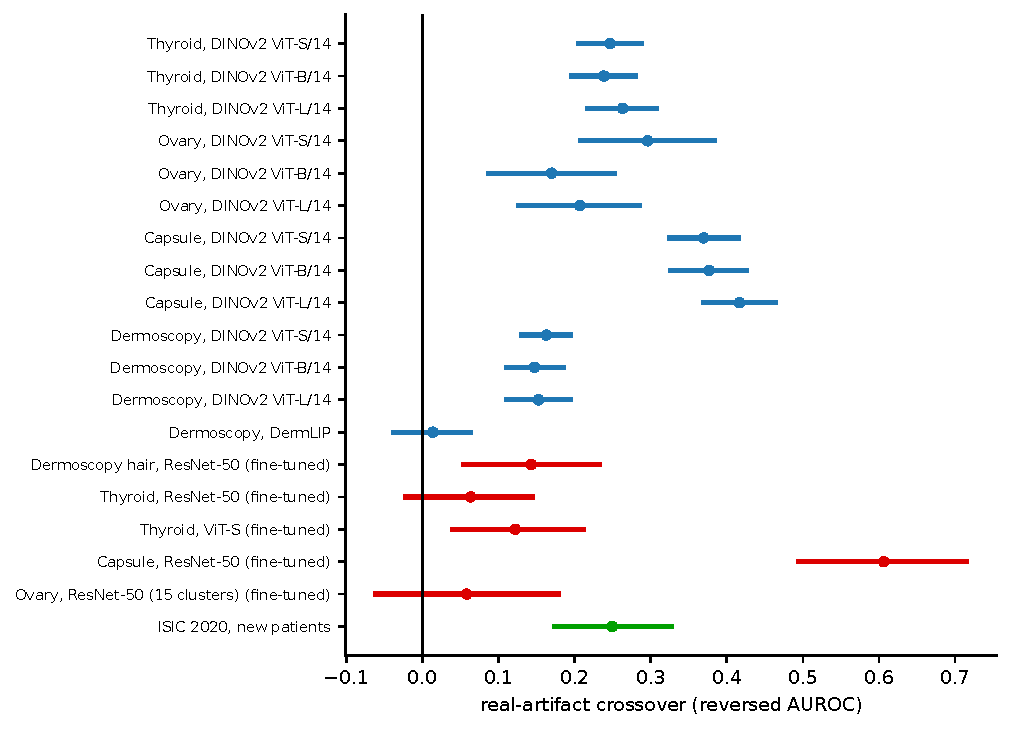
\includegraphics[width=0.8\linewidth]{../stage5_practice_theory/figures/breadth_forest.pdf}
\caption{Crossover across encoders and scales (blue), fine-tuned networks (red) and new patients (green); crossed 95\%
CIs.}\label{s5:fig:breadth}\end{figure}
\paragraph{Absolute performance} Table~\ref{s5:tab:lit}. On the one cohort with a published benchmark on the same
patient-disjoint split, the frozen DINOv2 linear probe reaches an AUROC of \sFiveLitOurs, below published fine-tuned CNNs
(0.77--0.80). The study is about the \emph{relative} effect of masking on a fixed representation, not about
state-of-the-art accuracy, but the gap is a limitation.
\begin{table}[H]\centering\scriptsize
\caption{Absolute performance: the frozen encoder with a linear head against published fine-tuned CNNs on the same patient-disjoint split.}\label{s5:tab:lit}
\begin{tabular}{lcc}\toprule
Model (thyroid, official TNCD test split) & AUROC & Source \\\midrule
ResNet-18, cross-entropy (fine-tuned) & 0.773 & \citet{gong2022acl} \\
DenseNet-121, cross-entropy (fine-tuned) & 0.780 & \citet{gong2022acl} \\
ConvNeXt-T, cross-entropy (fine-tuned) & 0.784 & \citet{gong2022acl} \\
ResNet-18, adaptive curriculum (fine-tuned) & 0.799 & \citet{gong2022acl} \\
DINOv2 ViT-B/14 frozen + linear head, ERM (rebuilt run) & 0.735 & this work \\
\bottomrule\end{tabular}
\end{table}


\subsubsection{The DermLIP exception}
With DermLIP, masking harms at both hair locations (Trap~A \sFiveDermmasktrapAtestrev, Trap~B \sFiveDermmasktrapBtestrev).
Two measurements explain it. First, masking costs DermLIP disease signal wherever the hair lies: clean-test AUROC changes by
\sFiveDermmasktrapAclean{} and \sFiveDermmasktrapBclean. Second, the pixel part of its hair shortcut is small at both
locations (oracle hair inpainting \sFiveDerminpainttrapAtestrev{} and \sFiveDerminpainttrapBtestrev), whereas group
balancing, which also removes correlates of hair, gains \sFiveDermbalancedtrapAtestrev{} and \sFiveDermbalancedtrapBtestrev:
DermLIP carries the hair shortcut mostly through correlates that masking does not remove at either location. In the terms
of the theory, masking lowers $S$ at both locations and removes little of $\tilde A$ at either, so there is no gap to
find. The theory anticipates this from the clean and correlated AUROC alone: predicted crossover \sFiveDermPred, observed
\sFiveDermObs.

\subsubsection{The theory, judged by held-out error}
\begin{figure}[H]\centering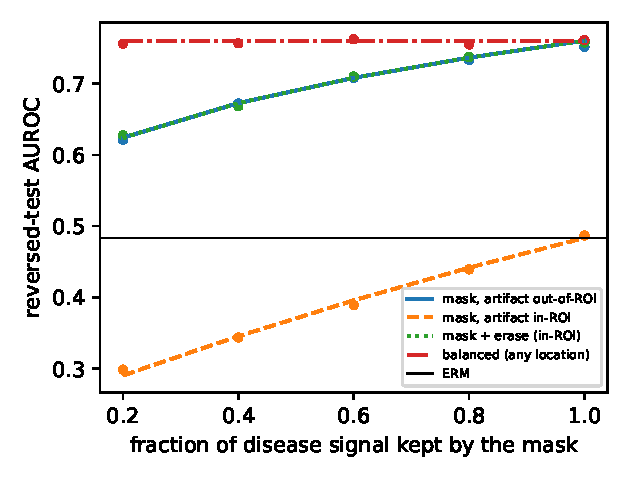
\includegraphics[width=0.55\linewidth]{../../paper/figures/theory.pdf}
\caption{The closed form (lines) against Monte Carlo simulation of its own model (points): the formula is exact up to
simulation noise (at most \sFiveSimMax{} AUROC over \sFiveSimN{} settings). This checks the algebra, not the
theory.}\label{s5:fig:sim}\end{figure}
Table~\ref{s5:tab:theory} and Figure~\ref{s5:fig:theory}. Over \sFiveTN{} primary cells the theory predicts the reversed AUROC
--- never used in fitting --- with mean absolute error \sFiveTMae{} (Pearson $r$ \sFiveTR; \sFiveTWithin{} within 0.05),
against \sFiveTMaeSym{} for the symmetric-reversal heuristic and \sFiveTMaeClean{} for ``reversed = clean''. It gets the
sign of all \sFiveTTwoN{} real-trap crossovers right (MAE \sFiveTTwoMae) and of \sFiveTTwoFt{} fine-tuned crossovers ---
networks that violate its assumptions --- and the sign of \sFiveTThreeSign{} of \sFiveTThreeN{} controlled-sweep gains
(heuristic: \sFiveTThreeSymSign). From the fitted $S$ alone, the sign of the in-ROI masking effect is right in
\sFiveTFourAgree{} of \sFiveTFourN{} cells. Its clear failure is the chest-drain cohort of Stage~3: the clean and
correlated environments do not reveal a shortcut carried by the treated lung, so the model cannot see it --- the boundary
its assumption (5) predicts.

The account is simple: a model's reliance on an artifact is fixed by the ratio of artifact to disease signal it sees;
masking lowers the disease signal (less context) and, when the artifact lies inside the ROI, leaves the artifact's signal
intact, so it raises that ratio exactly when the artifact is inside.
\begin{table}[H]\centering\scriptsize
\caption{Held-out prediction of the reversed-test AUROC (never used in fitting): the two-parameter theory fitted to each cell's clean and correlated AUROC, against two parameter-free heuristics.}\label{s5:tab:theory}
\begin{tabular}{lccccc}\toprule
Cells & Predictor & $n$ & MAE & Pearson $r$ & within 0.05 \\\midrule
Primary cells (ERM, mask) & linear-Gaussian theory & 136 & 0.052 & 0.914 & 66\% \\
 & heuristic: symmetric reversal & 136 & 0.129 & 0.743 & 40\% \\
 & heuristic: reversed = clean & 136 & 0.237 & 0.550 & 18\% \\
All ERM-head arms & linear-Gaussian theory & 598 & 0.036 & 0.933 & 79\% \\
 & heuristic: symmetric reversal & 598 & 0.076 & 0.823 & 65\% \\
 & heuristic: reversed = clean & 598 & 0.151 & 0.584 & 40\% \\
Fine-tuned (outside assumptions) & linear-Gaussian theory & 12 & 0.027 & 0.980 & 92\% \\
\bottomrule\end{tabular}
\end{table}

\begin{figure}[H]\centering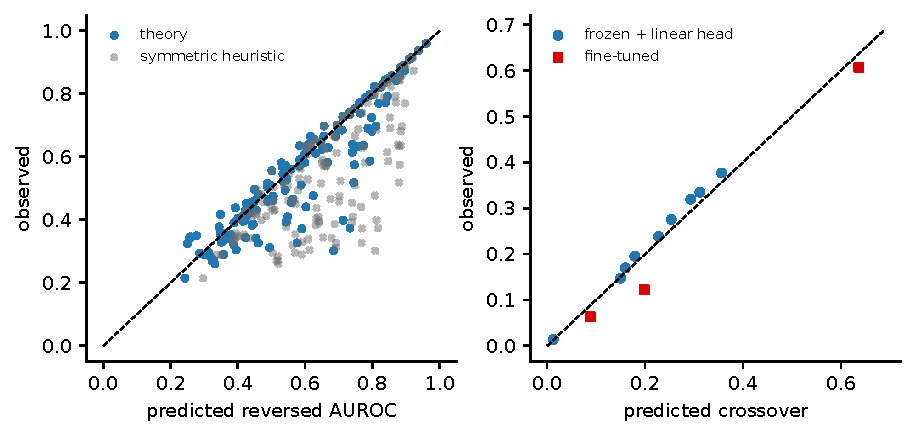
\includegraphics[width=\linewidth]{../stage5_practice_theory/figures/theory_prediction.pdf}
\caption{Left: predicted versus observed reversed AUROC (theory, blue; symmetric heuristic, grey). Right: predicted
versus observed real-trap crossover (frozen encoders, blue; fine-tuned, red).}\label{s5:fig:theory}\end{figure}
\paragraph{Verdict by the registered rule} The rule called the theory \emph{quantitatively predictive} only if every
crossover sign agreed, both correlations were $\ge0.7$, and its error beat ``reversed = clean''. On the full registered
cell set one near-zero chest-radiograph crossover (observed $\approx-0.002$) had the wrong sign; the report therefore calls
it a \emph{qualitative account that closely matches held-out results} and does not say that it ``predicts magnitudes''. The
correlation of predicted and observed crossovers ($r=$ \sFiveTTwoR) is not used as evidence, because the symmetric
heuristic also correlates almost perfectly; the held-out error is the evidence.

\subsubsection{Sensitivity to the interval estimator}
On the analyses of this stage (Table~\ref{s5:tab:estcheck}) the crossed intervals are wider by a median factor of
\sFiveEstMed; \sFiveEstLost{} of \sFiveEstN{} contrasts lose significance and \sFiveEstGained{} gains it
(Table~\ref{s5:tab:estchanges}). The ones that matter for the text --- masking's gain on the easy thyroid pairs and on all MSK
pairs --- are therefore not claimed; natural-set intervals are about twice as wide as the per-seed ones, because every seed
scores the same test images.
\begin{table}[H]\centering\scriptsize
\caption{The analyses of this stage under the per-seed and the crossed estimator (same predictions; baseline arms only).}\label{s5:tab:estcheck}
\begin{tabular}{p{5.0cm}p{1.4cm}p{2.6cm}p{2.6cm}p{2.4cm}}\toprule
Result group & Intervals & Excluded 0 only with the per-seed estimator & Excluded 0 only with the crossed estimator & Median width ratio (crossed / per-seed) \\\midrule
capsule/\allowbreak{}dinol518\_scale & 9 & 1 & 0 & 1.53 \\
capsule/\allowbreak{}dinos518\_scale & 9 & 0 & 0 & 1.38 \\
finetune/\allowbreak{}capsule & 4 & 0 & 0 & 1.10 \\
finetune/\allowbreak{}isic & 4 & 0 & 0 & 1.20 \\
finetune/\allowbreak{}ovary & 2 & 0 & 0 & 1.23 \\
finetune/\allowbreak{}thyroid & 8 & 1 & 1 & 1.17 \\
natural/\allowbreak{}capsule\_dino518\_repro & 6 & 0 & 0 & 1.16 \\
natural/\allowbreak{}isic\_BCN\_dino518\_repro & 6 & 0 & 0 & 1.72 \\
natural/\allowbreak{}isic\_HAM\_dino518\_repro & 6 & 0 & 0 & 1.95 \\
natural/\allowbreak{}isic\_MSK\_dino518\_repro & 6 & 2 & 0 & 2.01 \\
natural/\allowbreak{}thyroid\_dino518\_repro & 6 & 1 & 0 & 2.06 \\
ovary/\allowbreak{}dinol518\_scale & 9 & 1 & 0 & 1.58 \\
ovary/\allowbreak{}dinos518\_scale & 9 & 1 & 0 & 1.56 \\
spec\_e13/\allowbreak{}dinol518\_spec\_scale & 17 & 2 & 0 & 1.44 \\
spec\_e13/\allowbreak{}dinos518\_spec\_scale & 17 & 1 & 0 & 1.61 \\
thyroid/\allowbreak{}dinol518\_scale & 9 & 1 & 0 & 1.59 \\
thyroid/\allowbreak{}dinos518\_scale & 9 & 0 & 0 & 1.37 \\
zero\_shot/\allowbreak{}boot & 12 & 1 & 0 & 2.00 \\
\textbf{all} & 148 & 12 & 1 & 1.53 \\
\bottomrule\end{tabular}
\end{table}

\begin{table}[H]\centering\scriptsize
\caption{Contrasts of this stage whose verdict depends on the estimator.}\label{s5:tab:estchanges}
\begin{tabular}{p{4.2cm}p{5.2cm}p{3.3cm}p{2.6cm}}\toprule
Result & Contrast & Crossed estimate [95\% CI] & Verdict vs per-seed estimator \\\midrule
zero\_shot & medsiglip448 /\allowbreak{} ovary /\allowbreak{} trapB /\allowbreak{} zs\_mask-zs & $-0.054$ [$-0.135, +0.030$] & no longer excludes 0 \\
thyroid/\allowbreak{}dinol518\_scale & trapB /\allowbreak{} balanced /\allowbreak{} clean /\allowbreak{} balanced /\allowbreak{} erm & $+0.036$ [$-0.002, +0.073$] & no longer excludes 0 \\
ovary/\allowbreak{}dinos518\_scale & trapB /\allowbreak{} balanced /\allowbreak{} clean /\allowbreak{} balanced /\allowbreak{} erm & $+0.038$ [$-0.000, +0.077$] & no longer excludes 0 \\
ovary/\allowbreak{}dinol518\_scale & trapB /\allowbreak{} balanced /\allowbreak{} clean /\allowbreak{} balanced /\allowbreak{} erm & $+0.043$ [$-0.002, +0.087$] & no longer excludes 0 \\
capsule/\allowbreak{}dinol518\_scale & trapA /\allowbreak{} mask /\allowbreak{} clean /\allowbreak{} mask /\allowbreak{} erm & $+0.012$ [$-0.006, +0.031$] & no longer excludes 0 \\
spec\_e13/\allowbreak{}dinos518\_spec\_scale & trapB /\allowbreak{} mask /\allowbreak{} clean /\allowbreak{} all /\allowbreak{} mask /\allowbreak{} erm & $+0.028$ [$-0.000, +0.055$] & no longer excludes 0 \\
spec\_e13/\allowbreak{}dinol518\_spec\_scale & trapA /\allowbreak{} mask /\allowbreak{} test\_rev /\allowbreak{} HAM /\allowbreak{} mask /\allowbreak{} erm & $-0.044$ [$-0.090, +0.002$] & no longer excludes 0 \\
spec\_e13/\allowbreak{}dinol518\_spec\_scale & trapB /\allowbreak{} mask /\allowbreak{} clean /\allowbreak{} all /\allowbreak{} mask /\allowbreak{} erm & $-0.025$ [$-0.055, +0.003$] & no longer excludes 0 \\
natural/\allowbreak{}thyroid\_dino518\_repro & easy  /\allowbreak{}  mask-erm & $+0.042$ [$-0.011, +0.097$] & no longer excludes 0 \\
natural/\allowbreak{}isic\_MSK\_dino518\_repro & all  /\allowbreak{}  mask-erm & $+0.016$ [$-0.007, +0.038$] & no longer excludes 0 \\
natural/\allowbreak{}isic\_MSK\_dino518\_repro & all  /\allowbreak{}  balanced-mask & $-0.018$ [$-0.041, +0.005$] & no longer excludes 0 \\
finetune/\allowbreak{}thyroid/\allowbreak{}resnet50 & trapB /\allowbreak{} mask\_balanced /\allowbreak{} balanced & $+0.069$ [$-0.004, +0.143$] & no longer excludes 0 \\
finetune/\allowbreak{}thyroid/\allowbreak{}vit\_small\_patch16\_224.augreg\_in21k\_ft\_in1k & trapA /\allowbreak{} mask\_balanced /\allowbreak{} balanced & $+0.059$ [$+0.003, +0.122$] & now excludes 0 \\
\bottomrule\end{tabular}
\end{table}


\subsection{What failed or changed}
\begin{itemize}[leftmargin=*]\itemsep1pt
\item \textbf{Natural test sets}: N3 holds in three of five; HAM goes the other way and capsule is inconclusive.
\item \textbf{The thyroid subgroup} is a post hoc subgroup; its test was registered only after its AUROC result was known.
\item \textbf{Fine-tuning}: thyroid ResNet-50 is not significant; the ovary network is not evaluable.
\item \textbf{DermLIP}: no crossover; explained, and anticipated by the theory, but still an exception.
\item \textbf{The theory} is a qualitative account by its registered rule and fails for correlate-carried shortcuts (chest
drains); the chest-radiograph cells could not be re-estimated and are excluded from its current error figures.
\item \textbf{Absolute performance} is below task-specific fine-tuned models on thyroid.
\item \textbf{External validation is dermoscopy only}; no ultrasound or capsule cohort passed the gate.
\end{itemize}

\subsection{Anticipated questions}
\paragraph{Why does AUROC barely change on natural data while sensitivity drops by a quarter?} AUROC averages over all
positive--negative pairs, and most pairs do not involve the shortcut. A fixed threshold, however, is set on validation
data where the caliper helps; after masking the model's scores for malignant nodules without a supporting caliper fall
below it. The hard-pair AUROC and the subgroup sensitivity isolate exactly those cases.
\paragraph{Why does masking help on the hard HAM pairs?} This is not explained, and it is reported as a failure of N3
for that test set. A possible reading --- that for HAM-style images the model trained on BCN and MSK relied more on hair
beside the lesion than on hair on it, so that masking removed more shortcut than it kept --- has not been tested.
\paragraph{Why do larger models exploit the caliper more?} A plausible reading, not tested directly, is that they
represent small, high-contrast structures such as caliper crosses more distinctly (a larger $A$ in the theory), so the
linear head finds the shortcut more easily. What is established is only that scale is not a defence.
\paragraph{Why include zero-shot scores whose thyroid AUROC is at chance?} Only to show that the location effect lives in
the representation: even without any head trained on the trap, masking changes the artifact's influence differently
inside and outside the ROI.
\paragraph{Why is ISIC 2020 external if it is also ISIC?} It is a different acquisition campaign with different patients,
patient identifiers and no image overlap; the hair masks and lesion masks were produced by models frozen before any ISIC
2020 image was seen. It is external for patients, not for modality.
\paragraph{Is a two-parameter model with two inputs per cell not trivially accurate?} It has two inputs and predicts a
third quantity it never saw; the heuristics use the same two inputs and are two to four times worse. It also predicts
crossovers, which combine four cells, and signs of in-ROI effects.
\paragraph{Why keep the subgroup result if it is post hoc?} It is the clinically meaningful case --- a malignant nodule the
sonographer measured --- and the test in it was registered before it was computed. It is labelled exploratory everywhere.

\subsection{Conclusion}
\textbf{Supported.} On unaltered data masking harms the shortcut-conflicting cases in three of five test sets and lowers
thyroid sensitivity at every validation-fixed operating point (registered decision rule met). The crossover replicates
across encoder families and sizes, in three of the four evaluable fine-tuned networks, in untrained vision--language
scores and on new patients. A two-parameter theory matches held-out reversed AUROC far better than heuristics, explains
every regime observed so far, and anticipates the DermLIP exception. \textbf{Qualified.} The \sFiveNConf-nodule subgroup
is exploratory confirmation; the theory is a qualitative account by its own rule. \textbf{Not supported.} Harm on natural
HAM and capsule test sets; a crossover for DermLIP and for the thyroid ResNet-50.

\subsection{Questions for the supervisor}
\begin{enumerate}\itemsep1pt
\item Is a sensitivity loss on one patient-disjoint split (thyroid) enough for a clinical claim, or should the thesis
lead with the AUROC on shortcut-conflicting cases?
\item Should the theory be a main contribution (with its held-out error as evidence) or a supporting section?
\item Is ISIC 2020 enough external validation, given that it is the same modality and artifact as the main dermoscopy
analysis?
\item Should the below-benchmark absolute performance of frozen linear probes be addressed with fine-tuned models in the
main text, or is the fine-tuned replication sufficient?
\end{enumerate}

